\documentclass[report.tex]{subfiles}
\begin{document}
\clearpage
\subsection{Results}
\label{sec:lab2_results}
The simulation results for chapter \ref{sec:lab2} is summarized below

\begin{figure}[h]
    \centering
    \subfloat[Resistor]{
        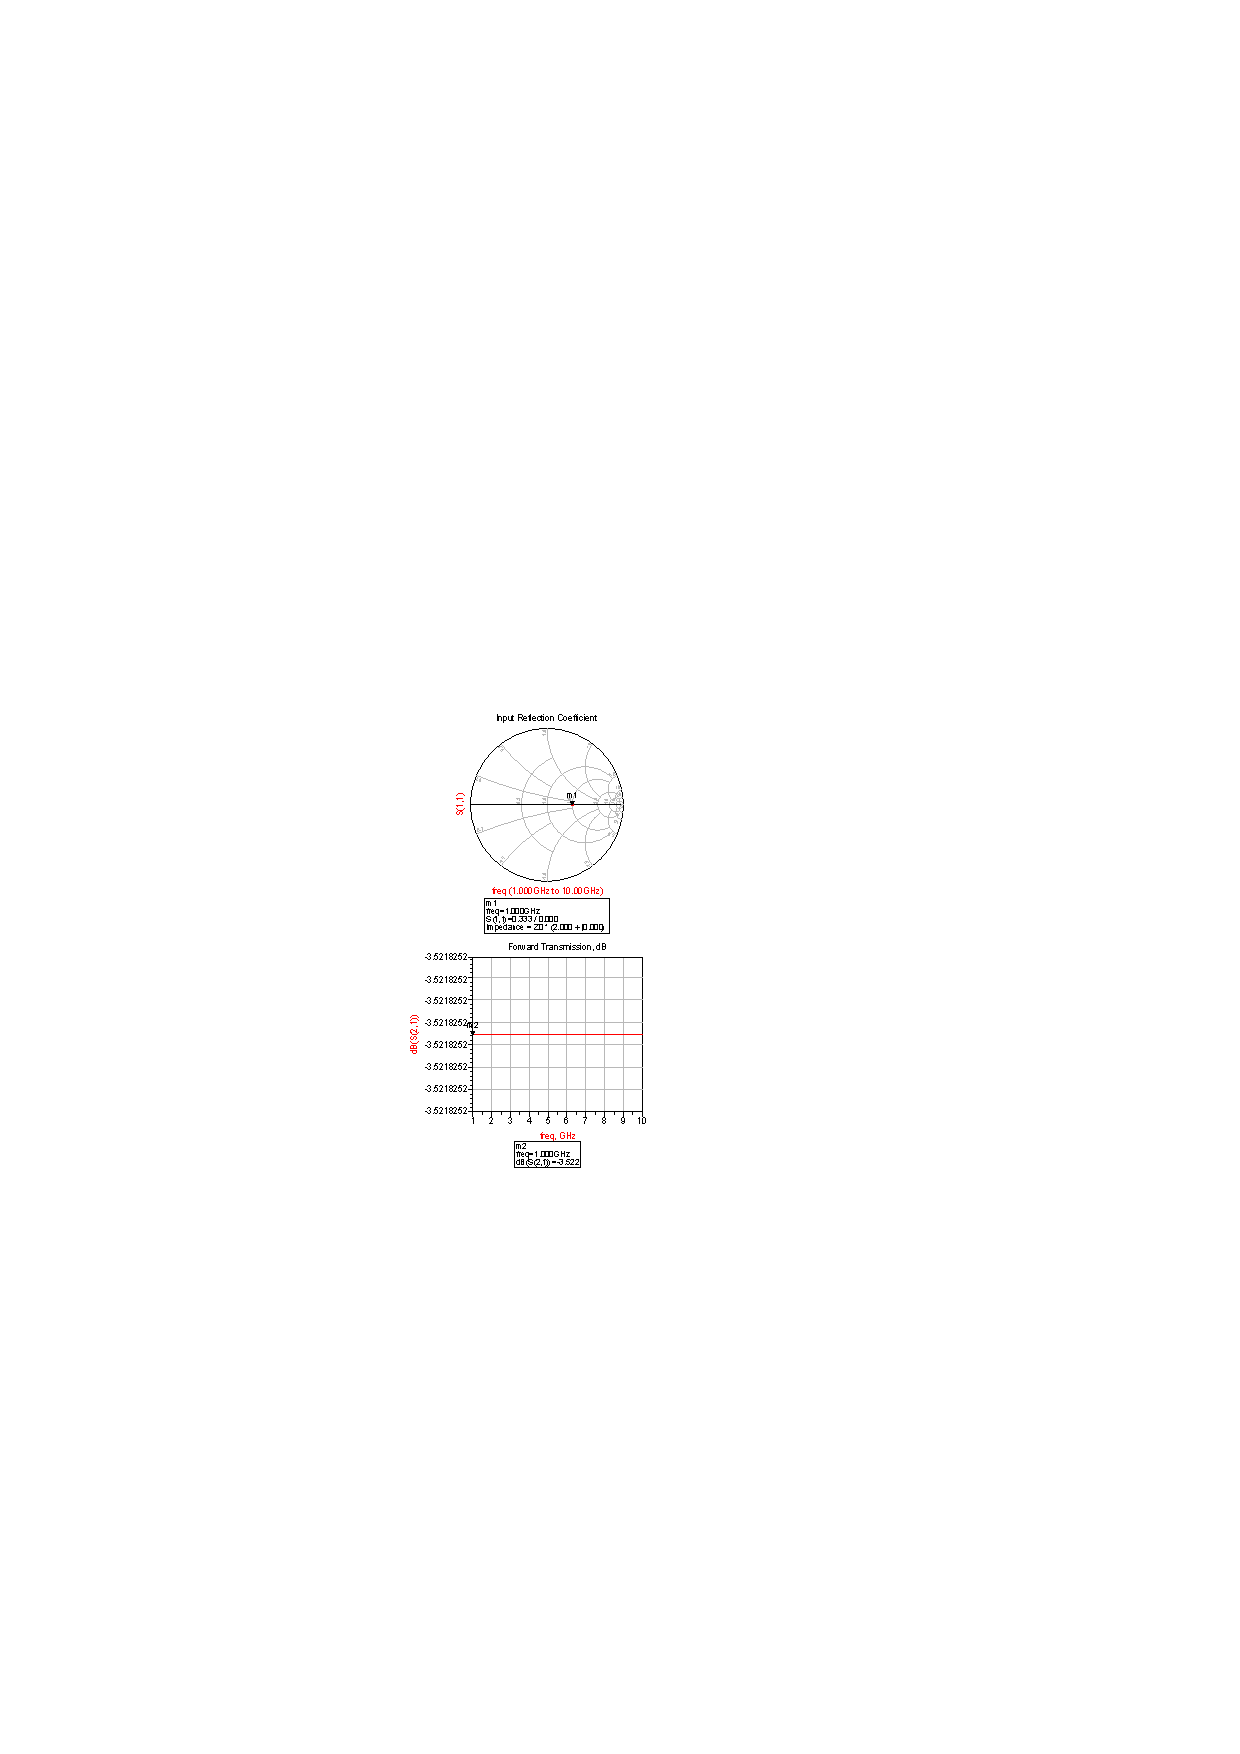
\includegraphics[scale=1.2]{S-params_50ohm_resistor}
    }
    \subfloat[Capacitor]{
        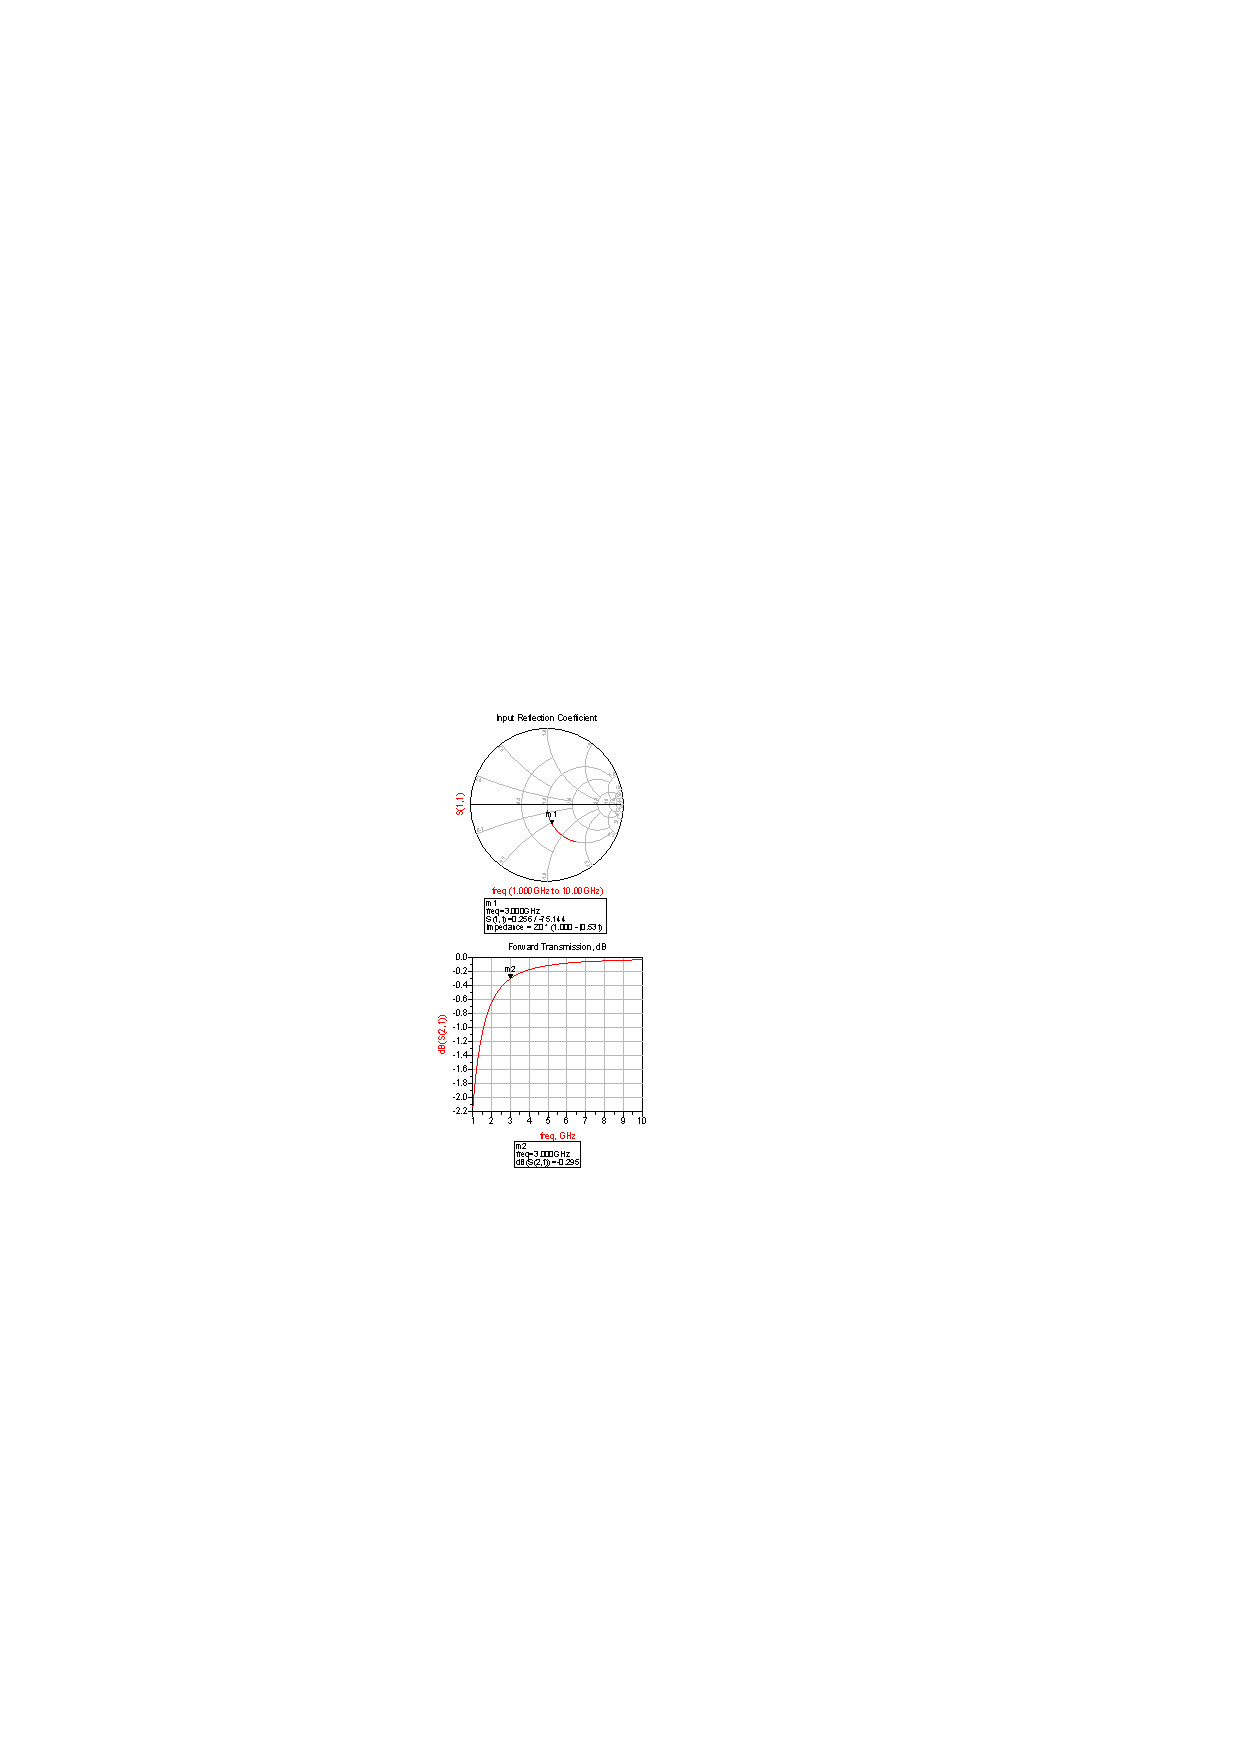
\includegraphics[scale=1.2]{S-params_2pF_capacitor}
    }
    \subfloat[Inductor]{
        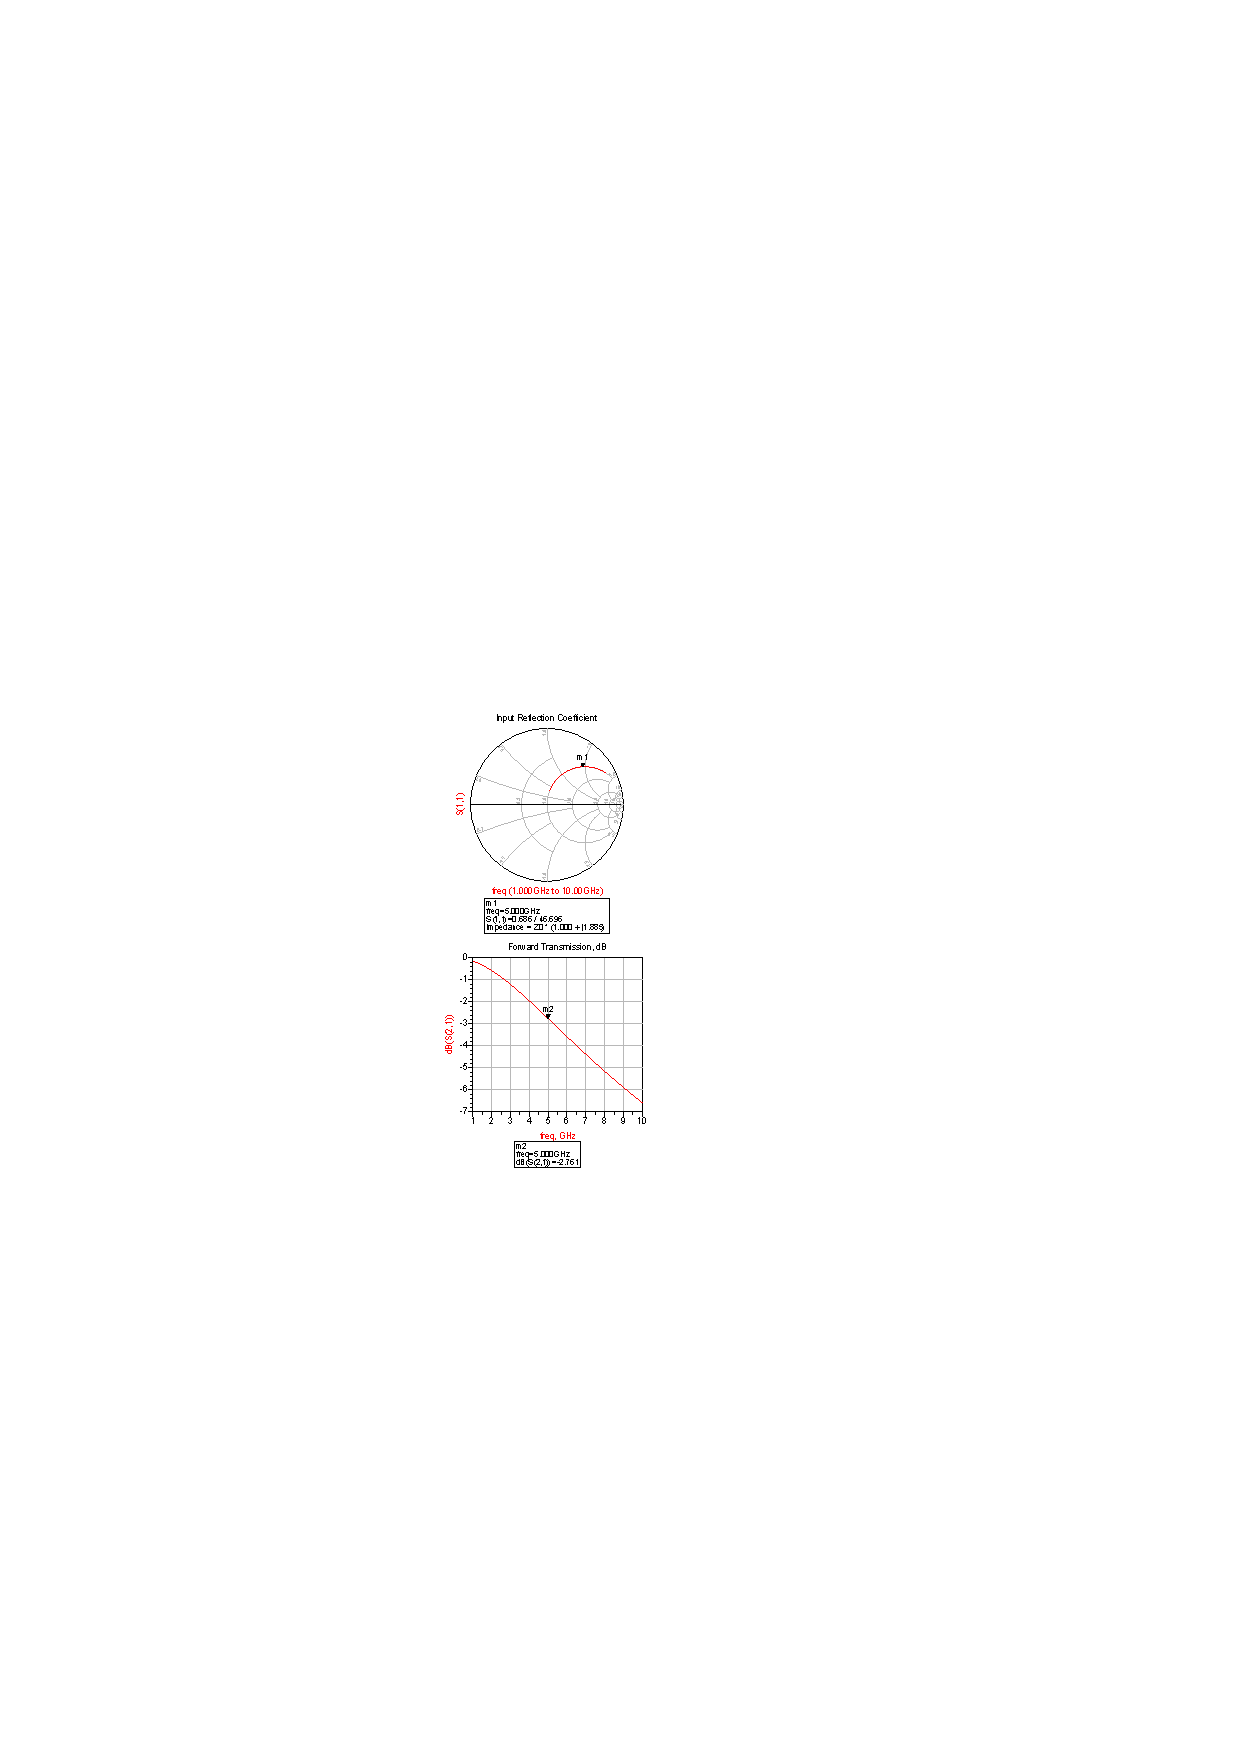
\includegraphics[scale=1.2]{S-params_3nH_coil}
    }
    \caption{Simulation results of three basic components}
\end{figure}
\clearpage

%\begin{figure}
%    \centering
%    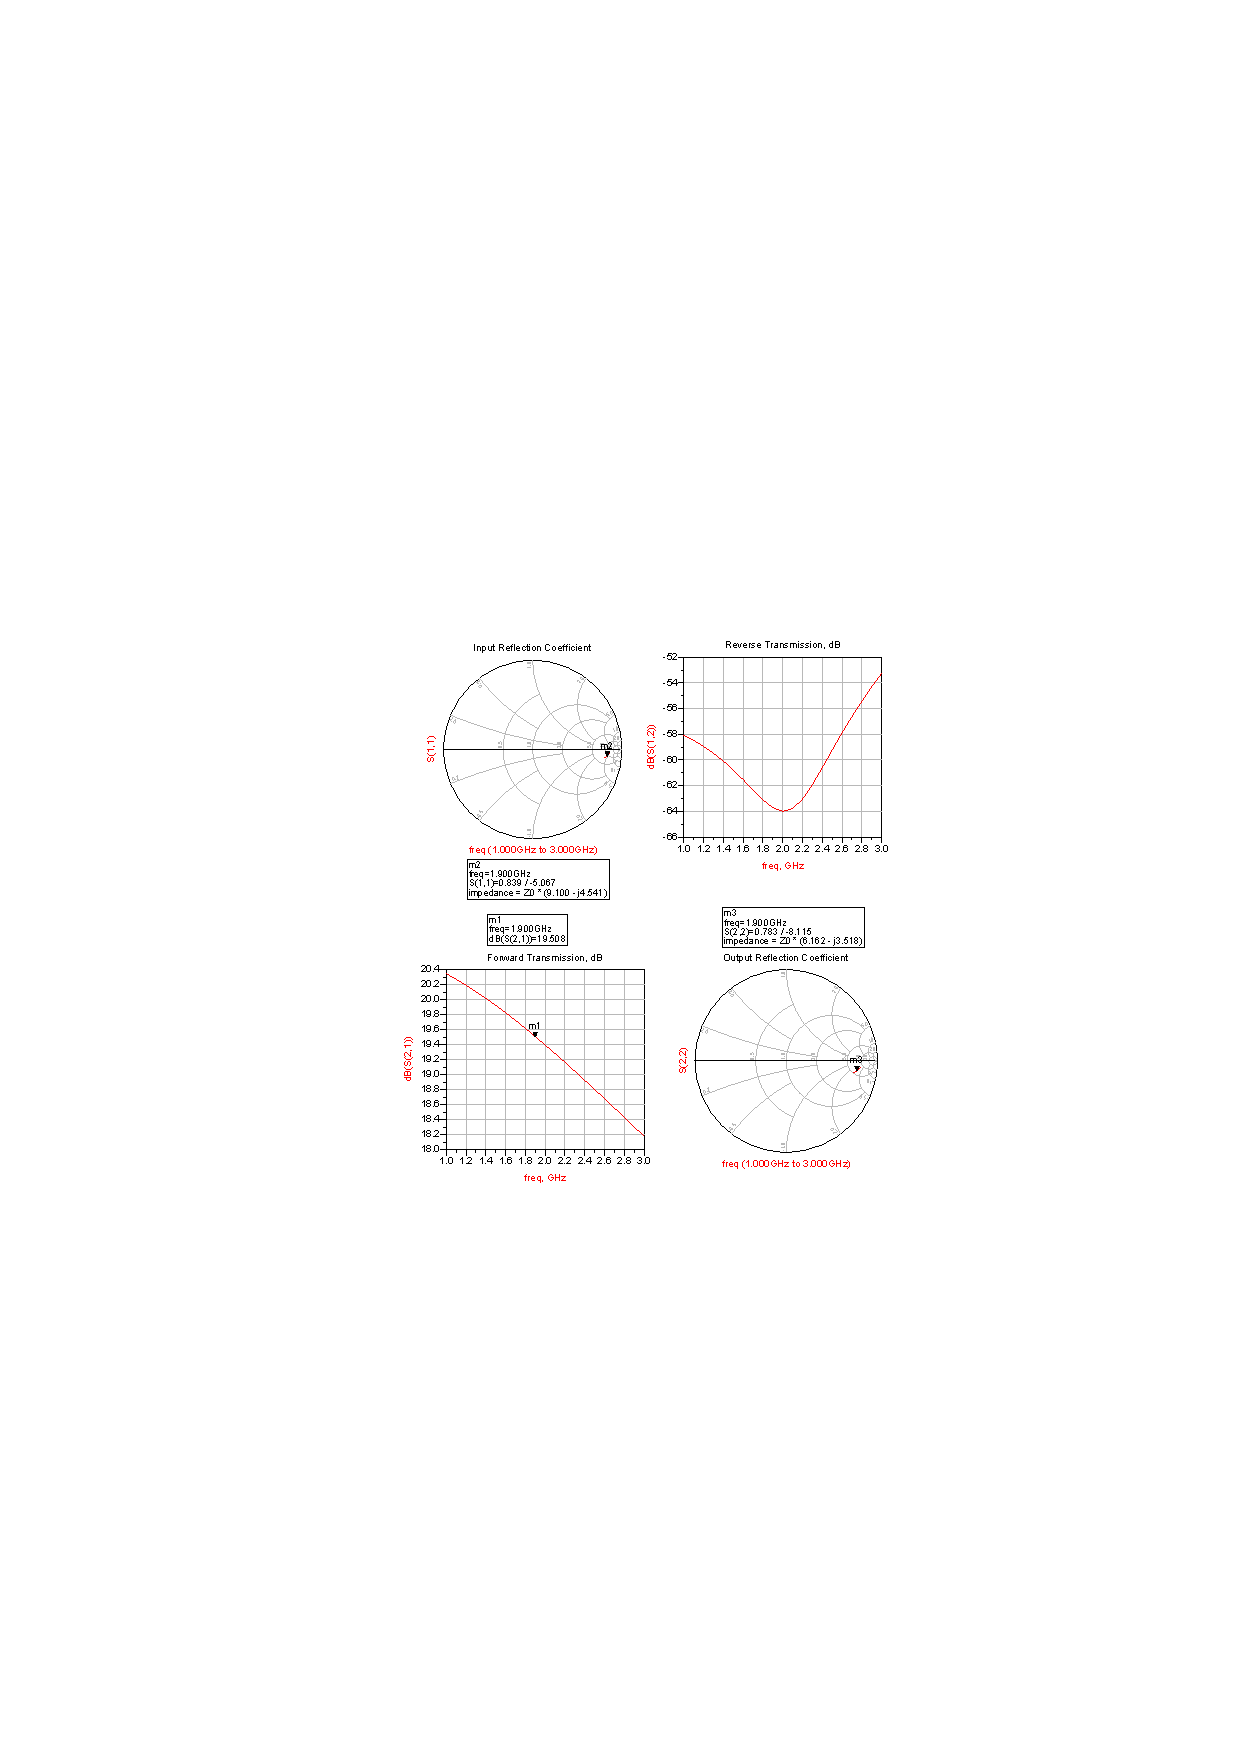
\includegraphics[width=0.8\linewidth]{S-params_unmatched_NPN}
%    \caption{S-parameters vs. frequency of unmatched NPN transistor}
%\end{figure}
%\begin{table}
%    \centering
%    \caption{Summare of input and output parameters}
%    \begin{tabular}{l l l}
%        $Z_{in} [\Omega]$ & $Z_{out} [\Omega]$ & $S_{21} [dB]$\\
%        \hline
%        $455-j227$  & $308-j176$  & 19.5 \\
%    \end{tabular}
%\end{table}
\clearpage

\begin{figure}
    \centering
    \subfloat[]{
        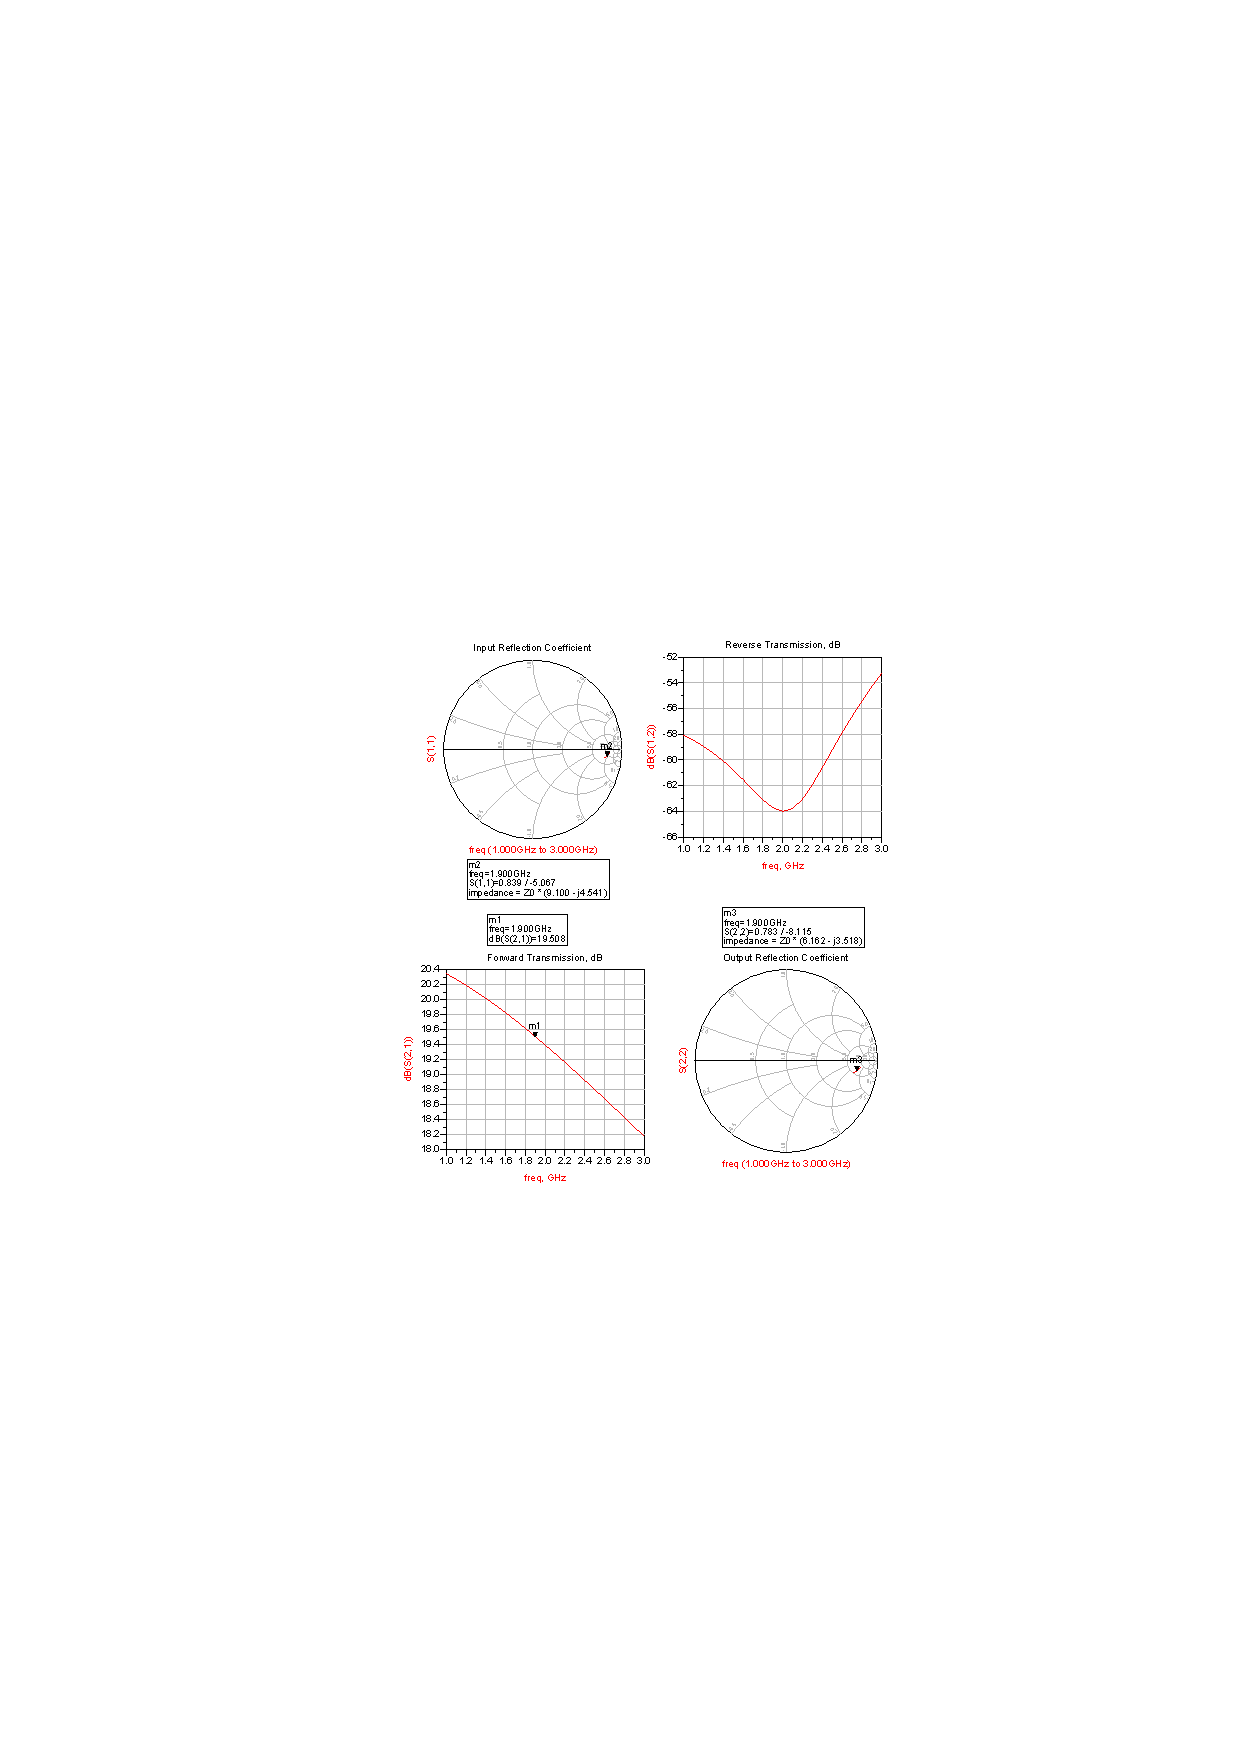
\includegraphics[width=0.5\linewidth]{S-params_unmatched_NPN}
    }
    \subfloat[]{
        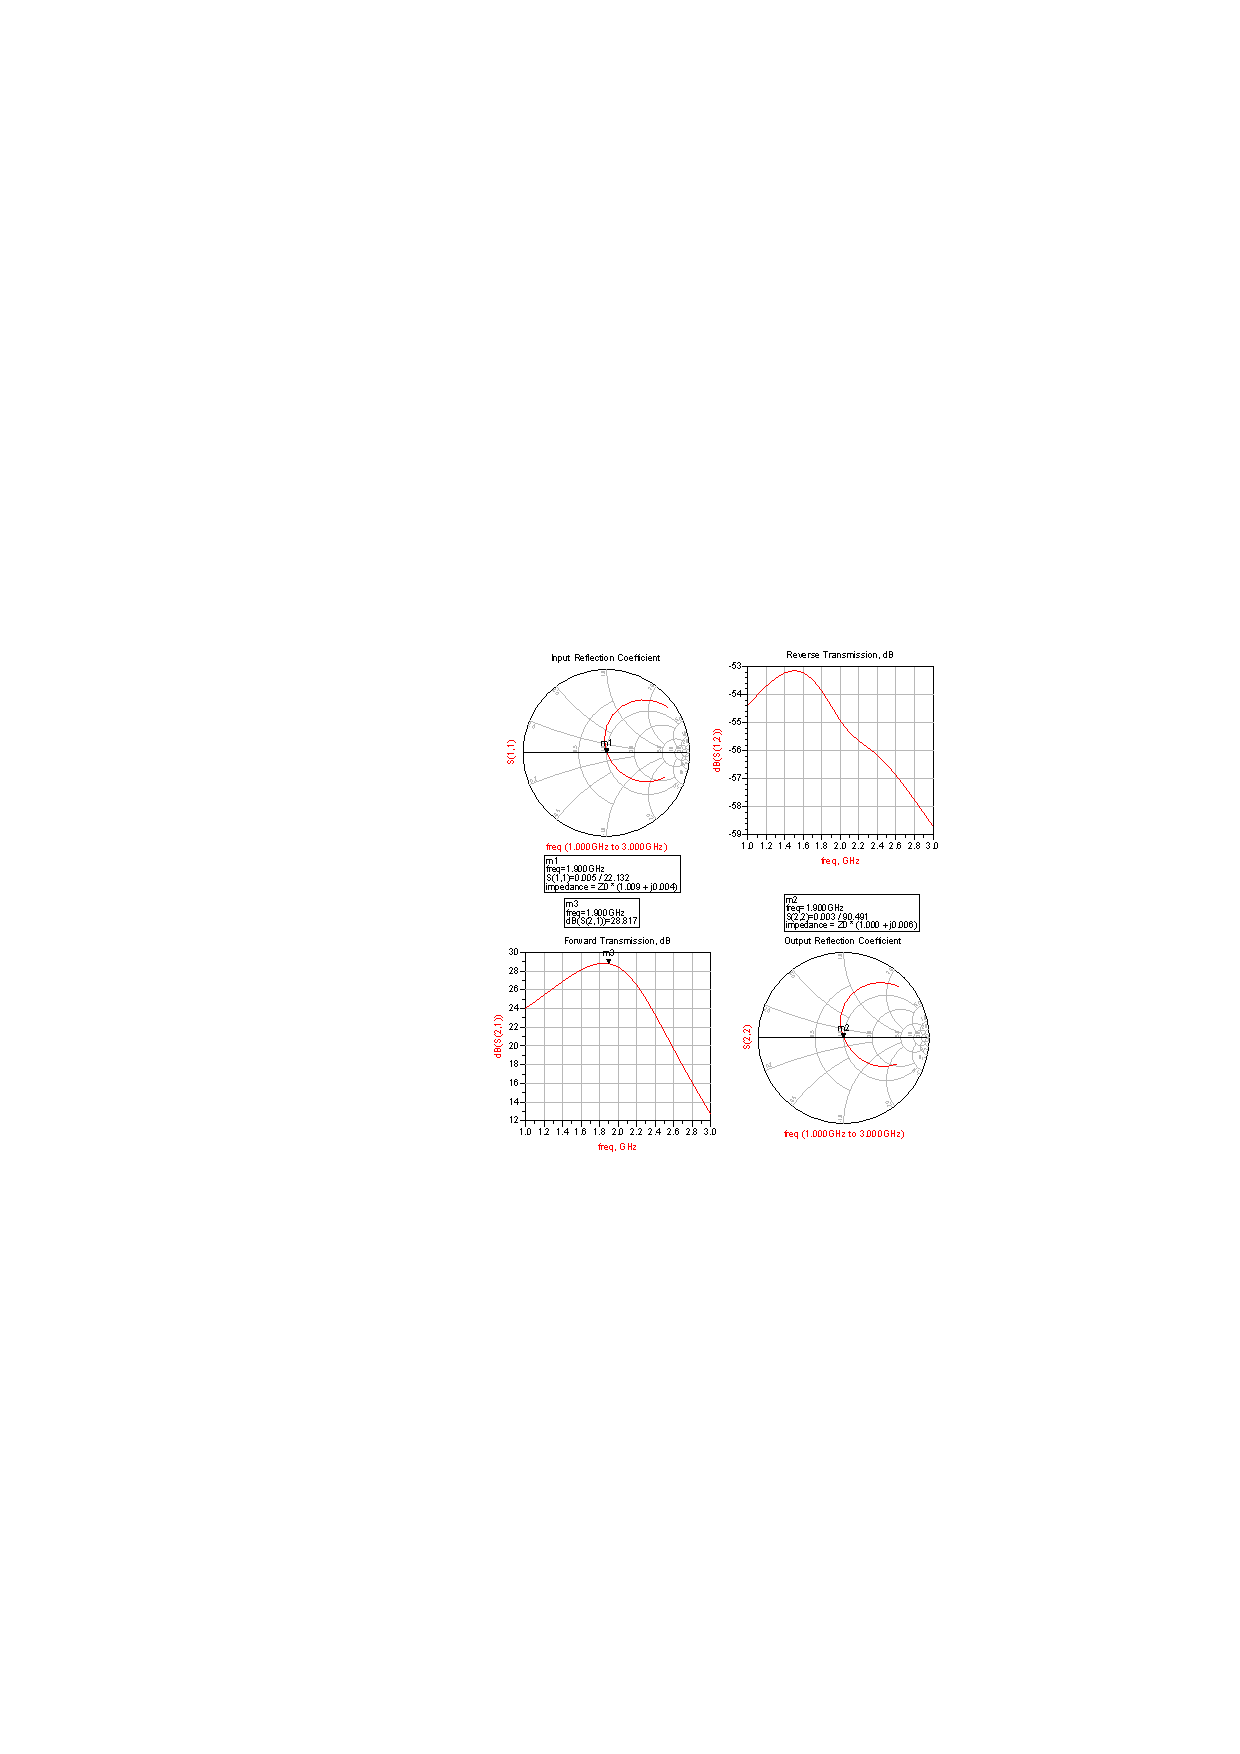
\includegraphics[width=0.5\linewidth]{S-params_matched_NPN}
    }
    \caption{S-parameters of an (a) un-matched and (b)matched NPN transistor}
\end{figure}

%\begin{figure}
%    \centering
%    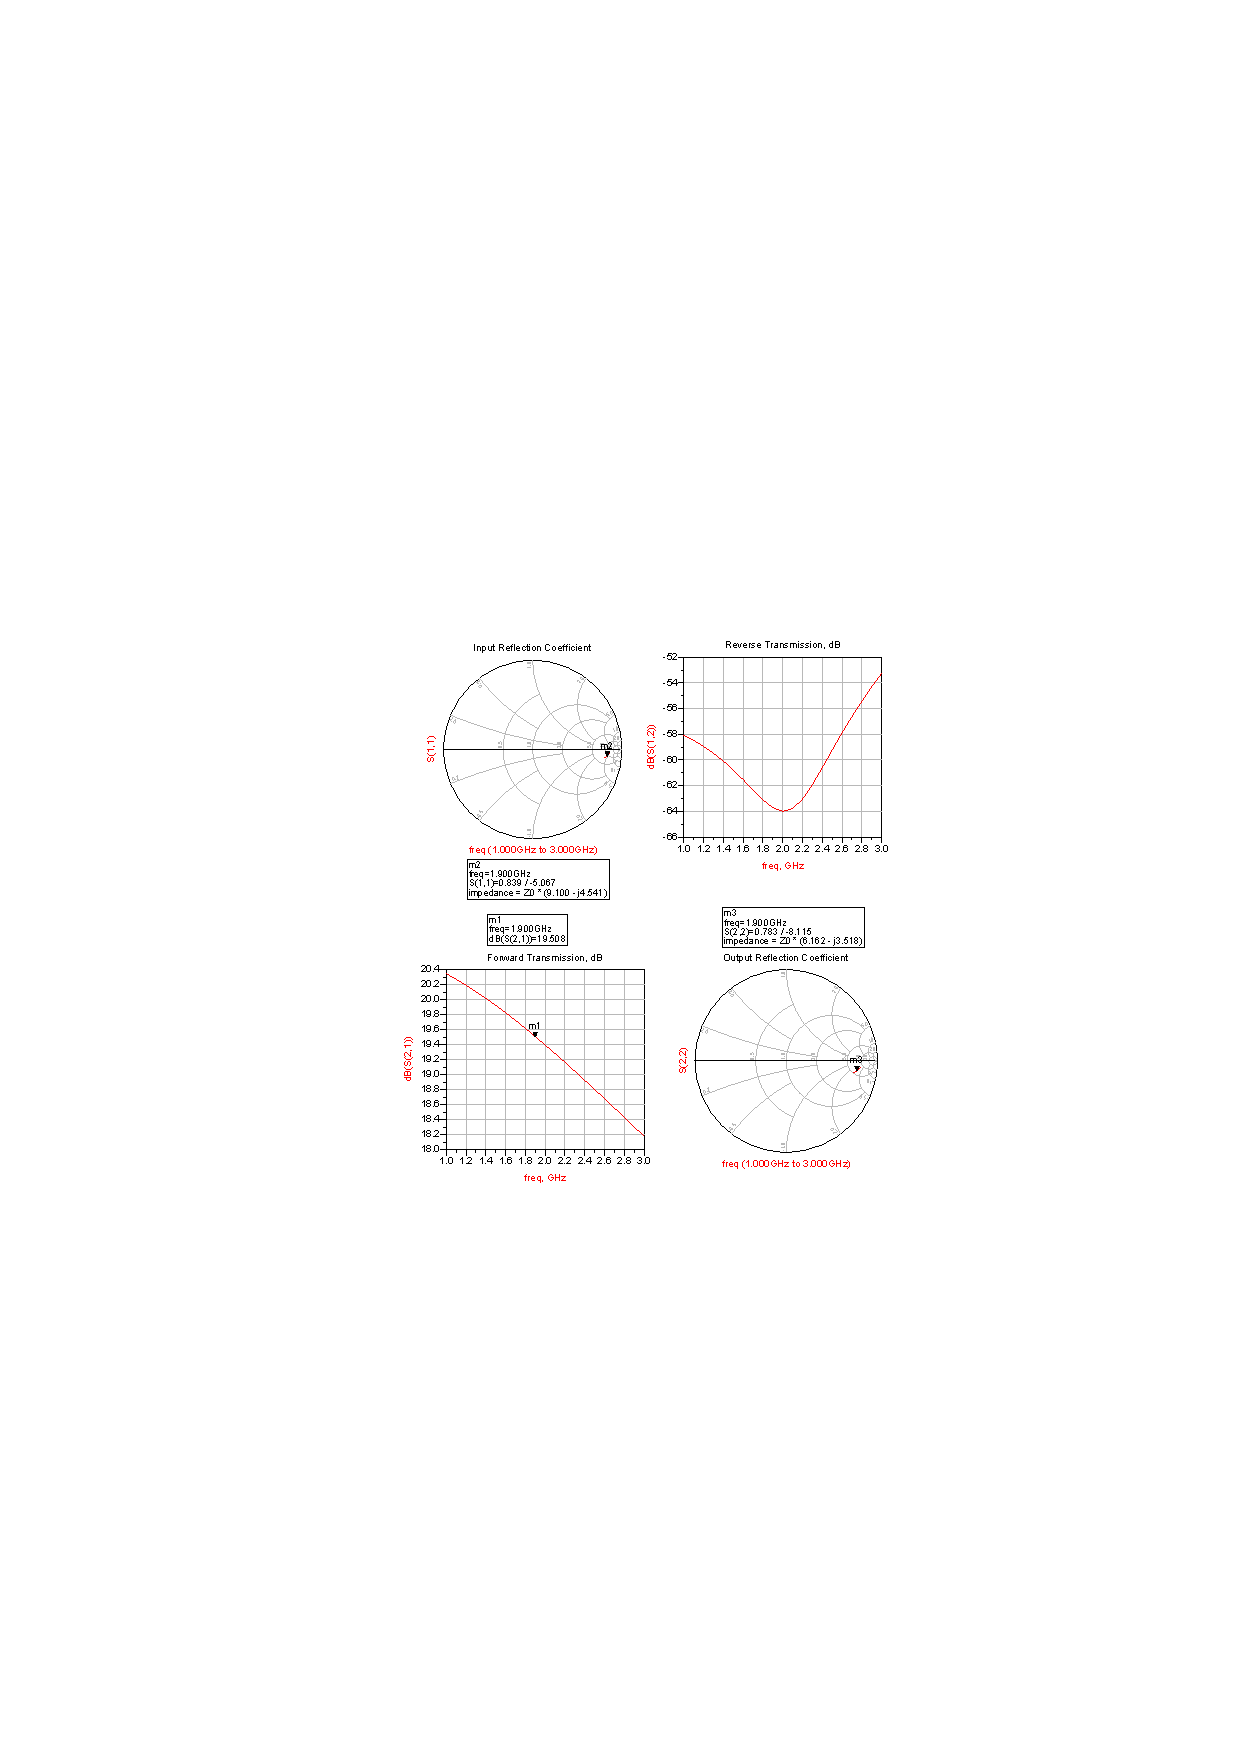
\includegraphics[width=0.8\linewidth]{S-params_unmatched_NPN}
%    \caption{S-parameters vs. frequency of un-matched NPN transistor}
%\end{figure}
%\clearpage
%
%\begin{figure}
%    \centering
%    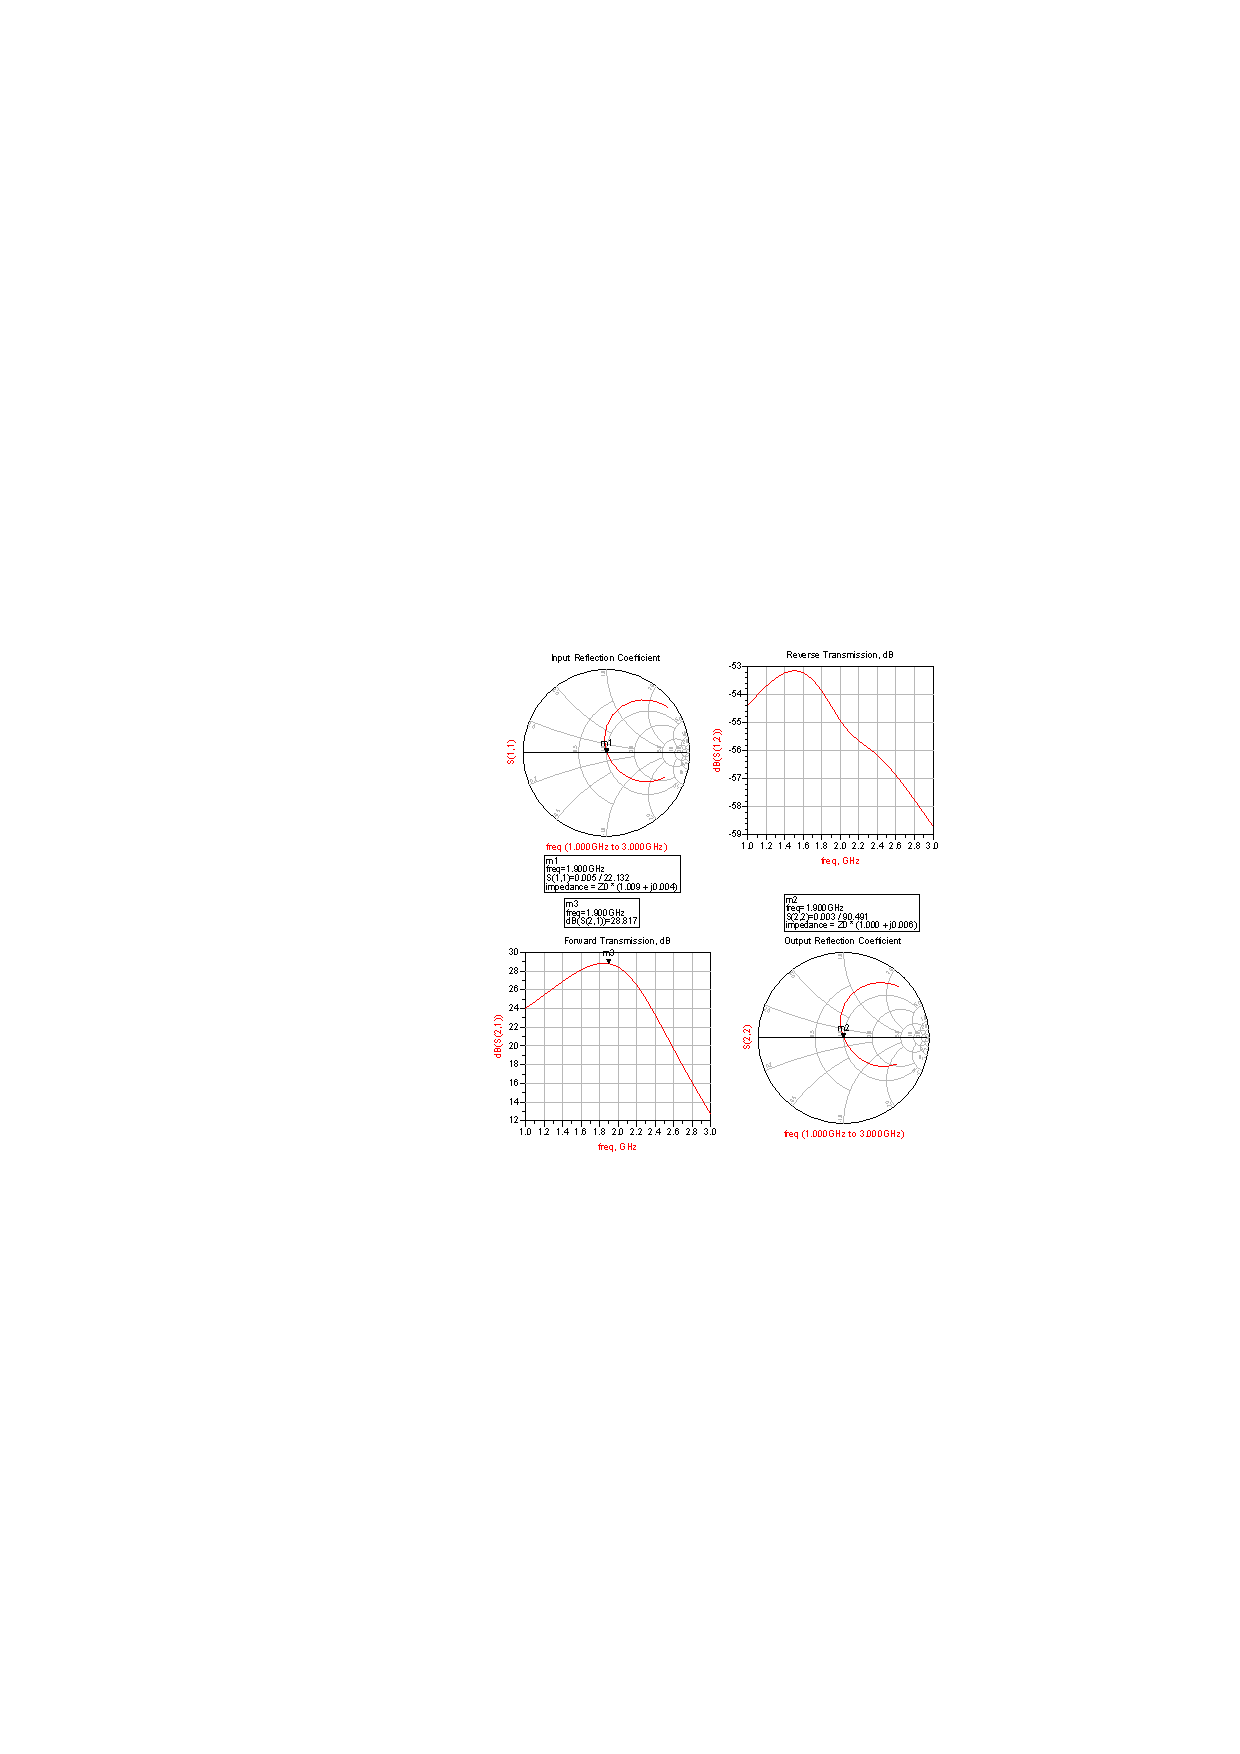
\includegraphics[width=0.8\linewidth]{S-params_matched_NPN}
%    \caption{S-parameters vs. frequency of impedance matched NPN transistor}
%\end{figure}

\begin{table}
    \centering
    \caption{Summary of input and output parameters}
    \begin{tabular}{l | l l l}
        & $Z_{in} [\Omega]$ & $Z_{out} [\Omega]$ & $S_{21} [dB]$\\
        \hline
        Un-matched & $455-j227$  & $308-j176$  & 19.5 \\
        Matched    & $50.5+j0.2$ & $50.0+j0.3$ & 28.8 \\
    \end{tabular}
\end{table}

\clearpage

\end{document}